\subsection{Prototype}

From the list of features mentioned in the previous chapter we have selected the most important ones and created a prototype in a form of MVP (Minimum Viable Product). 

The selected features:

\begin{enumerate}
	\requirement{3}{load an Instruction}
	\requirement{3}{view the 3D representation of the Instruction step}
	\requirement{3}{switch to the next step in the Instruction}
	\requirement{3}{switch to the previous step in the Instruction}
	\requirement{3}{see the Transition between two Instruction steps}
	\requirement{2}{pause the Transition at any time}
	\requirement{2}{rewind the Transition}
	\requirement{2}{forward the Transition}
	\requirement{3}{rotate the Model in 3D space}
	\requirement{3}{zoom the Model in and out in 3D space}
	\requirement{1}{see creases of the Model} 
	\requirement{2}{distinguish paper's top and bottom sides} 
\end{enumerate}

Some of the listed functionalities require a numerical solver which is also included in the MVP.

Both Instructions and Transitions are represented using .fold files which we have extended with information required by the application.

\subsubsection{Frontend}

At first we had decided to use plain \tech{JavaScript} with the \tech{Rollup} bundler and \tech{Three.js} framework.
It quickly became apparent that the lack of state management will become problematic as the development progresses. Following that realization we have decided to incorporate a reactive framework - \tech{React} to aid the project with basic layout and aforementioned state manipulation. 
Due to minor interoperability issues the Rollup was also replaced with \tech{Webpack}.

The quality assurance is achieved through the use of:

\begin{description}
\item[Code linter] - EsLint
\item[Code prettiefier] - Prettier
\item[Test Runner] - Jest
\item[Continuous integration] - Github Actions
\end{description}

The implementation is continuously delivered to \tech{Netlify} via Github Actions.


\begin{figure}[H]
\caption{Origami simulation view}
  \centering
    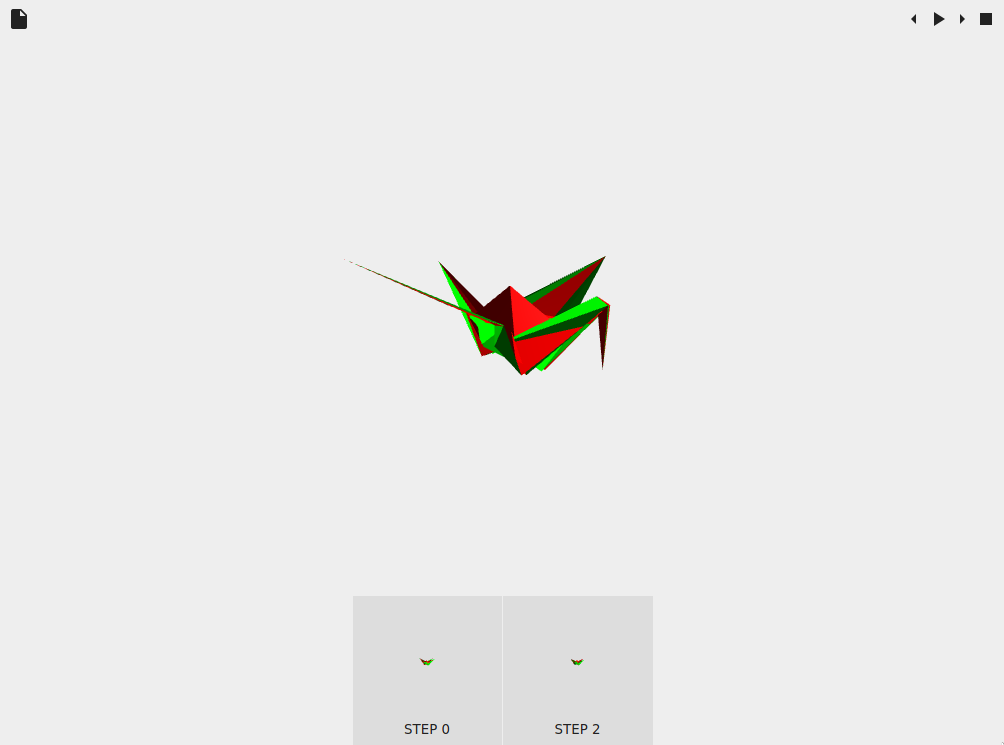
\includegraphics[width=0.8\textwidth]{assets/prototype-front.png}
\end{figure}

\subsubsection{Backend}

The current backend part is responsible for carrying out numerical computations.
It converts a provided Instruction into a set of coordinates representing
transitions between folding steps.\\

The solver is based on the techniques presented in the publication by A. Ghassaei.\cite{origami-simulator:paper}.

The computational framework consists of the three most important forces,
that drive the folding process.

\begin{description}
	\item[Beam force] - responsible for preserving edge length
	\item[Face force] - responsible for preserving the original face shape
	\item[Crease force] - responsible for folding
\end{description}

Given the current vertices' positions, and the mountain-valley assignment,
the solver computes forces imposed on vertices, and calculates their next position
using the forward Euler integration.

An additional \textbf{damping force} is introduced to prevent solver from
high frequency oscilations, assuring numerical stability under most conditions.\\

The solver is implemented in \tech{python}, using \tech{numpy} and \tech{scipy} libraries. 


\begin{figure}[H]
	\caption{Visualization of vertices (dots), and forces applied to them (arrows)
	during folding of a rectangular sheet of paper in half, along the diagonal. }
  \centering
    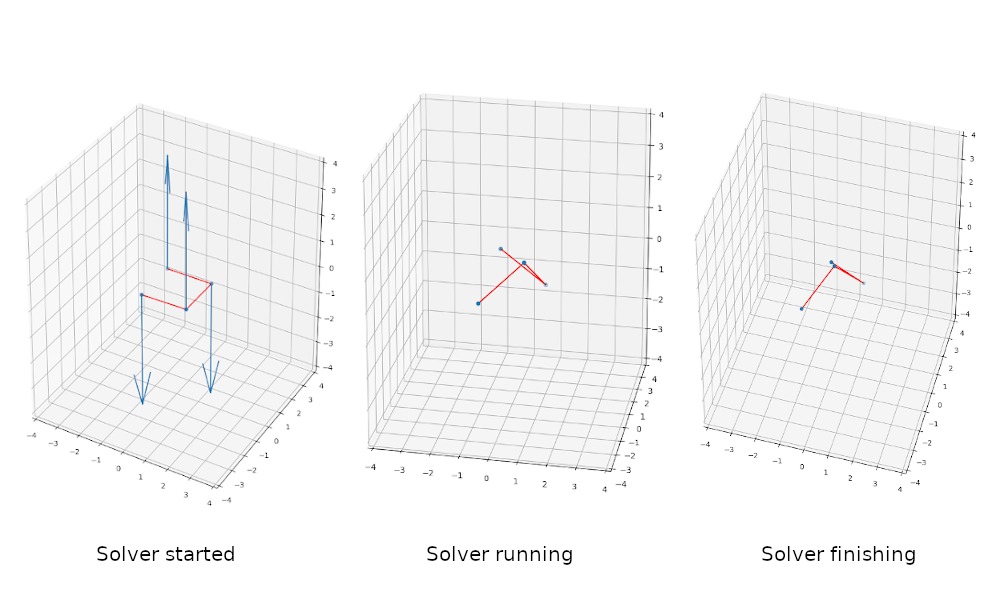
\includegraphics[width=0.8\textwidth]{assets/prototype-backend.png}
\end{figure}


\subsection{Project overview}

\begin{figure}[H]
	\caption{High level system overview}
  \centering
    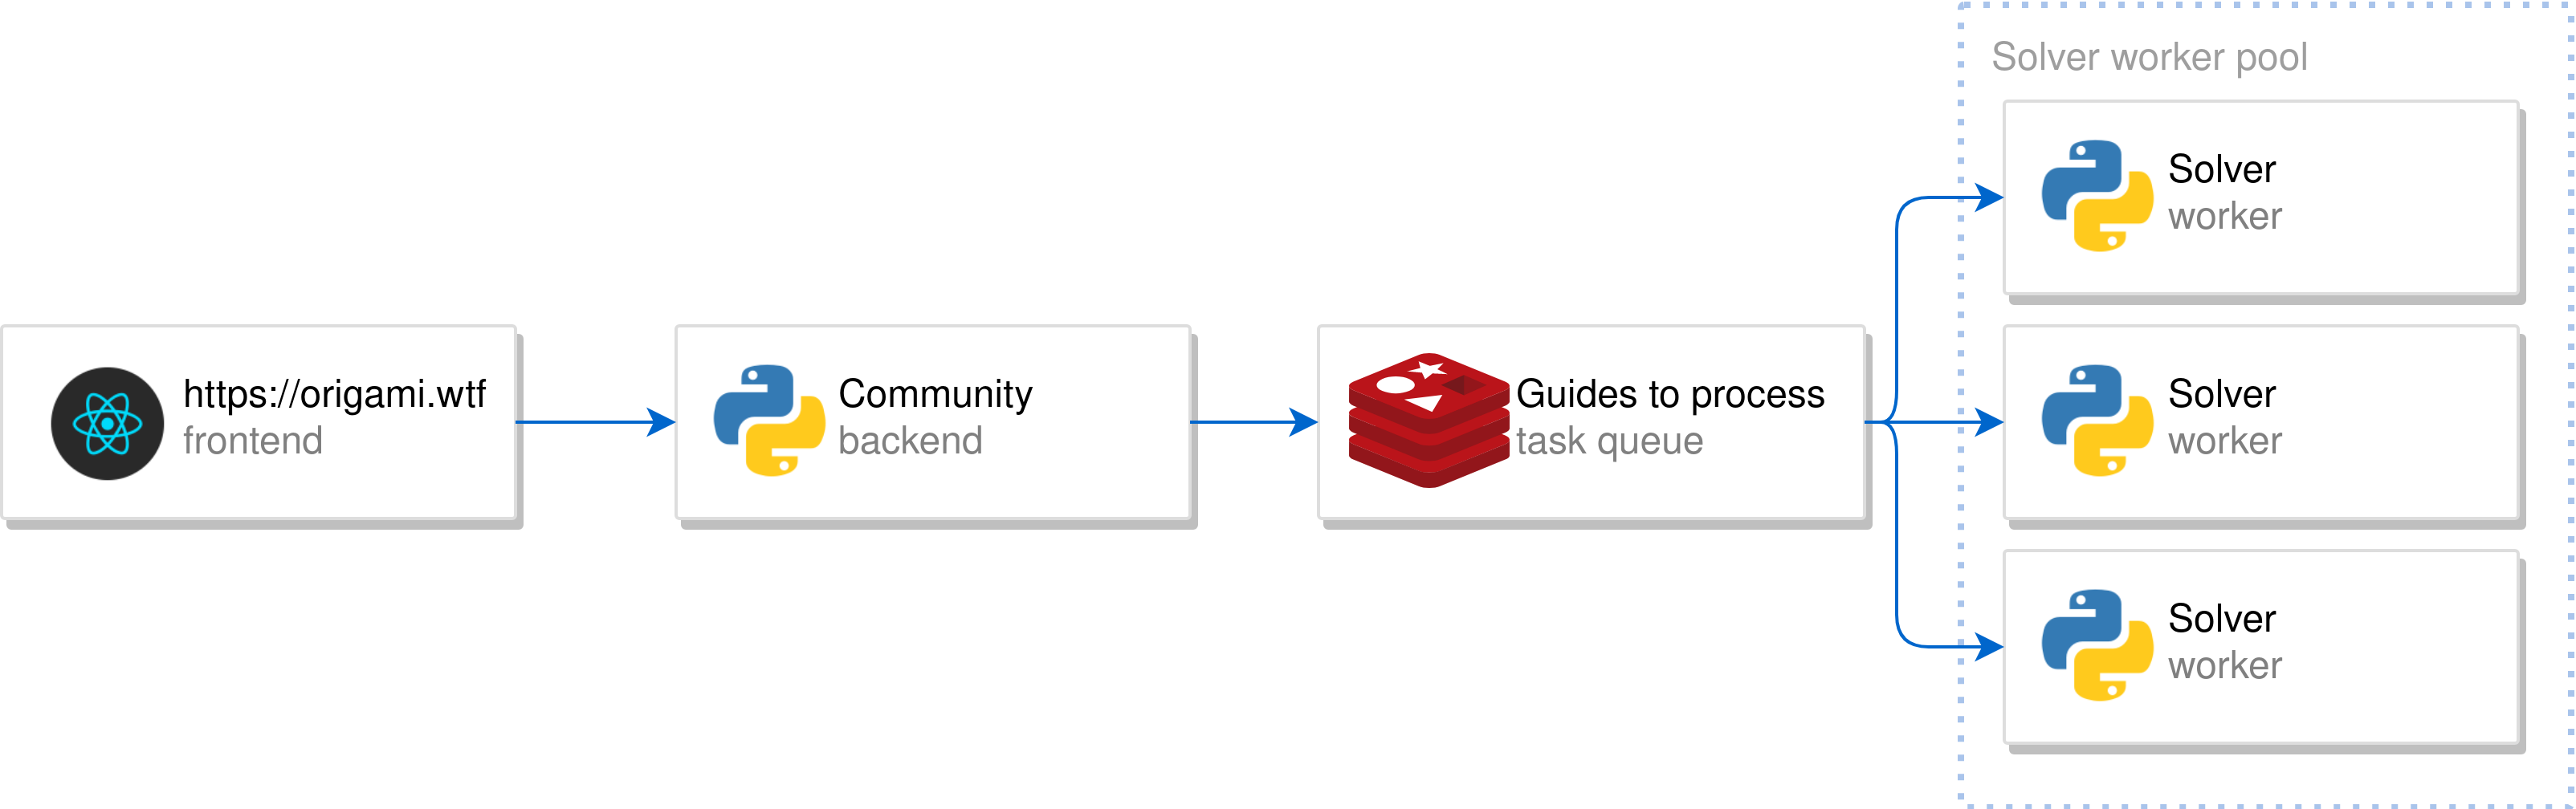
\includegraphics[width=\textwidth]{assets/architecture.png}
\end{figure}

Origuide consists of the following layers:
\begin{description}
	\item[Frontend] - a component that handles all user interactions with the system. 
	\item[Backend] - a component responsible for: \begin{itemize}
		\item processing all user requests initiated on the Frontend
		\item managing persistent data 
		\item authentication and authorization
		\item scheduling Guide processing
	\end{itemize}
	\item[Guides to process] - a task queue distributing guides to process among Solver workers
	\item[Solver worker] - a component responsible for converting Instructions to Guides.
\end{description}

As we previously distinguished two types of users in the system, there are two main success paths through the application.

\begin{figure}[H]
	\caption{Designer's success path}
  \centering
    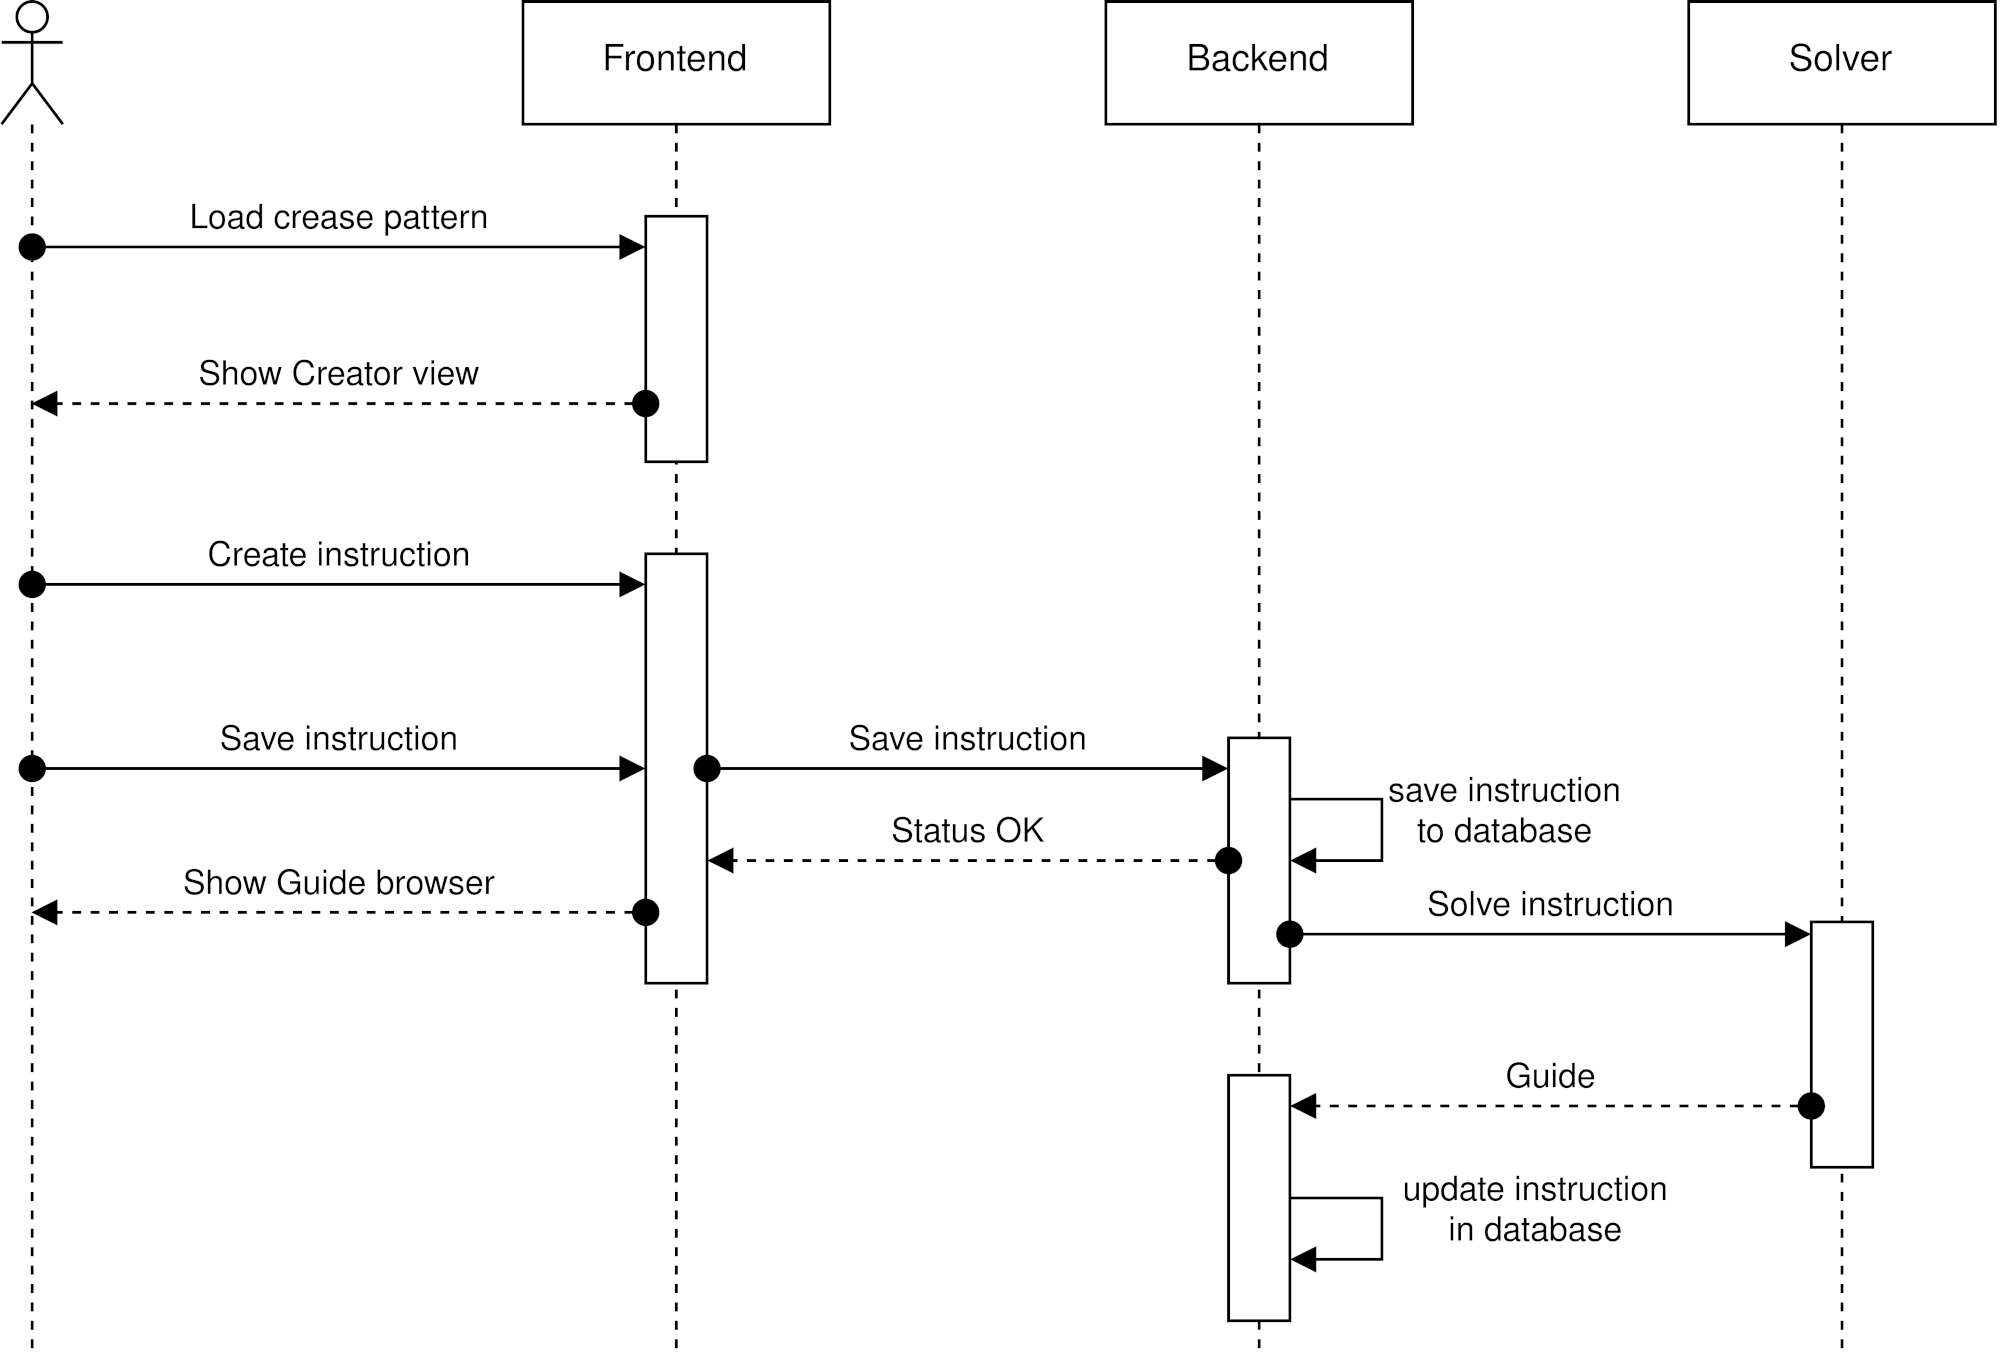
\includegraphics[width=\textwidth]{assets/3-designer-flow.png}
\end{figure}

Designer's main objective is to create Guides. After uploading a Crease Pattern, Designer is required to provide Instruction steps. When an Instruction is saved it gets scheduled on a Task Queue and processed by a Solver worker. Once processing is finished the Instruction associated with the Guide is marked as solved in the database.

\begin{figure}[H]
	\caption{Folder's success path}
  \centering
    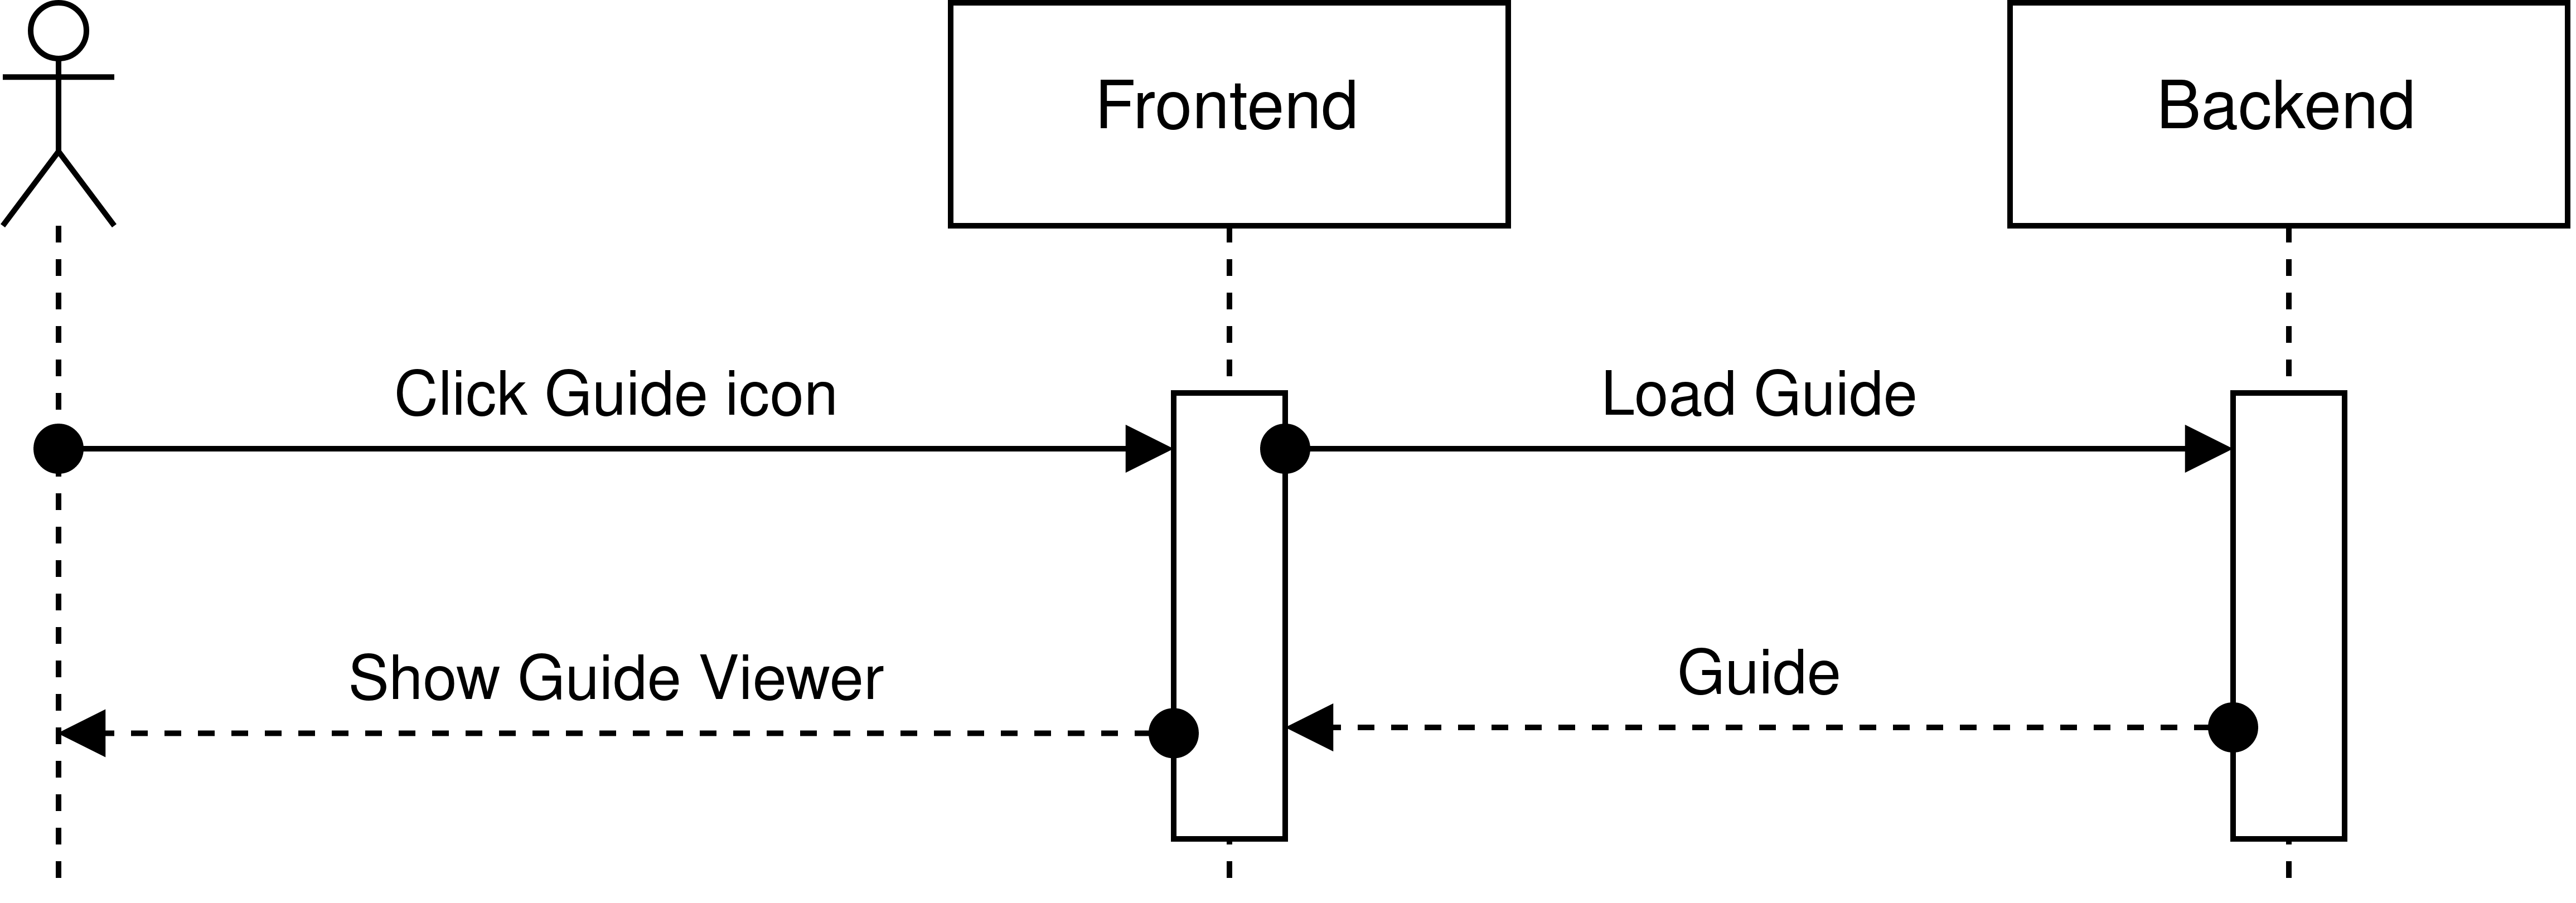
\includegraphics[width=\textwidth]{assets/3-folder-flow.png}
\end{figure}

Folder's main objective is to fold origami figures following steps presented by the Application. After successfully retrieving a guide from the Backend, he is presented with a Guide Viewer.

\subsection{Technology stack}

Source Code is version controlled using a hosted \tech{Git} solution - \tech{Github}.  

Continuous Integration and Continuous Deployment is provided by \tech{Github Actions}. 

\subsubsection{Frontend}

\begin{itemize}
	\item The Application is built in \tech{Javascript} using \tech{React} framework. 
	\item \tech{Three.JS} is used to display 3D models.
	\item Triangulation is done using \tech{earcut}. 
	\item Parsing folds is aided by \tech{fold}.
	\item User Interface components come mainly from \tech{material-ui}.
	\item \tech{Webpack} is responsible for bundling, minimizing and transpiling the source code.
	\item Code style is checked using \tech{Prettier} with \tech{eslint} and enforced on every commit using \tech{Husky}.
	\item \tech{Jest} has been incorporated as a test runner.
\end{itemize}

// TODO: comment

\subsubsection{Backend}

\begin{itemize}
	\item The Backend is built in \tech{Python} using \tech{Django} framework. 
	\item \tech{DjangoRestFramework} simplifies a REST server setup.
	\item \tech{drf-base64} helps with decoding of base64 encoded files.
	\item \tech{PyJWT} assists in auth process.
	\item \tech{factory-boy} is used to generate testing data.
	\item Data is stored in a \tech{PostgreSQL} database.
	\item \tech{Celery} was chosen for an asynchronous task processing.
	\item \tech{Redis} acts as a task queue for \tech{Celery}.
\end{itemize}


\subsubsection{Solver}

\begin{itemize}
	\item Solver runs under \tech{Python}'s alternative implementation - \tech{PyPy}.
	\item \tech{Shapely} is used for triangulation.
\end{itemize}



\subsection{Components overview}
% Przegląd poszczególnych komponentów a wiec np. baza danych, aplikacja typu klient, serwis RESTowy. Jeśli baza to ERD z opisem, jeśli aplikacja kliencka to jakie elementy, widoki, jak się łączy i kiedy. Jeśli prosta aplikacja WWW to można pokazać strukturę projektu. Jeśli serwis RESTowy to jego specyfikacja z przykładami. Protokół komunikacji to może być zupełnie osobny opis. %

\subsection{Algorithms}
% Ciekawsze algorytmy, aspekty, mechanizmy np. logowanie, indeksowane, cachowanie, synchronizacja, backup, jakieś procesy w tle, jakieś progress bary, jakieś analizy, generowanie warstw GISowych, lokalizacja etc. Jest tu często o czym pisać. %

\subsubsection{Solver}

\textit{Please note that most of the ideas in this section come from \cite{origami-simulator:paper}}.
\smallskip

The input to the Solver is a \textit{.fold} file containing an Instruction, and its output is a \textit{.fold} file containing a Guide. 
Instruction, at its simplest, is a set of vertices laying on a flat surface, and a set of edge assignments in each step.
The Solver's job is to output a resulting Guide file which has all the information necessary to display
a folding animation - that is, all the vertex positions at each step in time.

\smallskip
\textbf{Triangulation}
\smallskip

The Solver works using only triangular faces.
Therefore, before any folding-algorithm can happen, it has to generate a mesh that only consists of triangles.
\begin{figure}[H]
    \centering
    \subfloat[\centering Crease pattern before triangulation]{{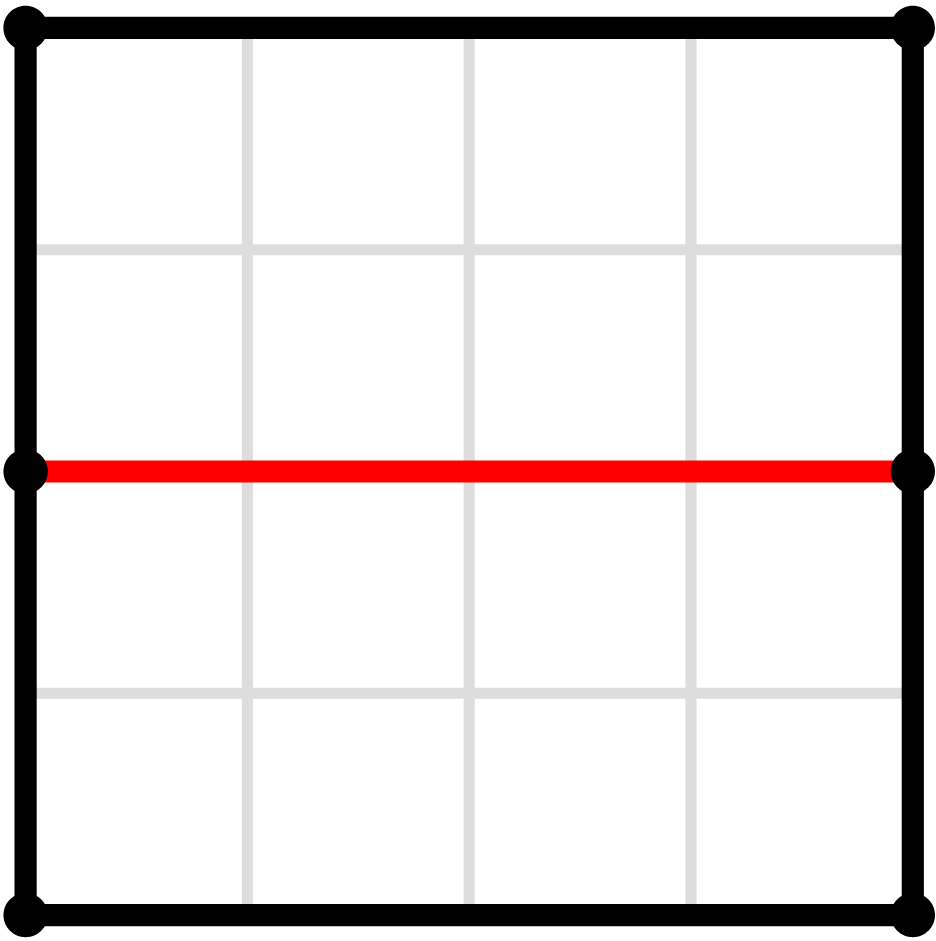
\includegraphics[width=.4\linewidth]{assets/3-2d-cp.png} }}
    \qquad
    \subfloat[\centering Crease pattern after triangulation]{{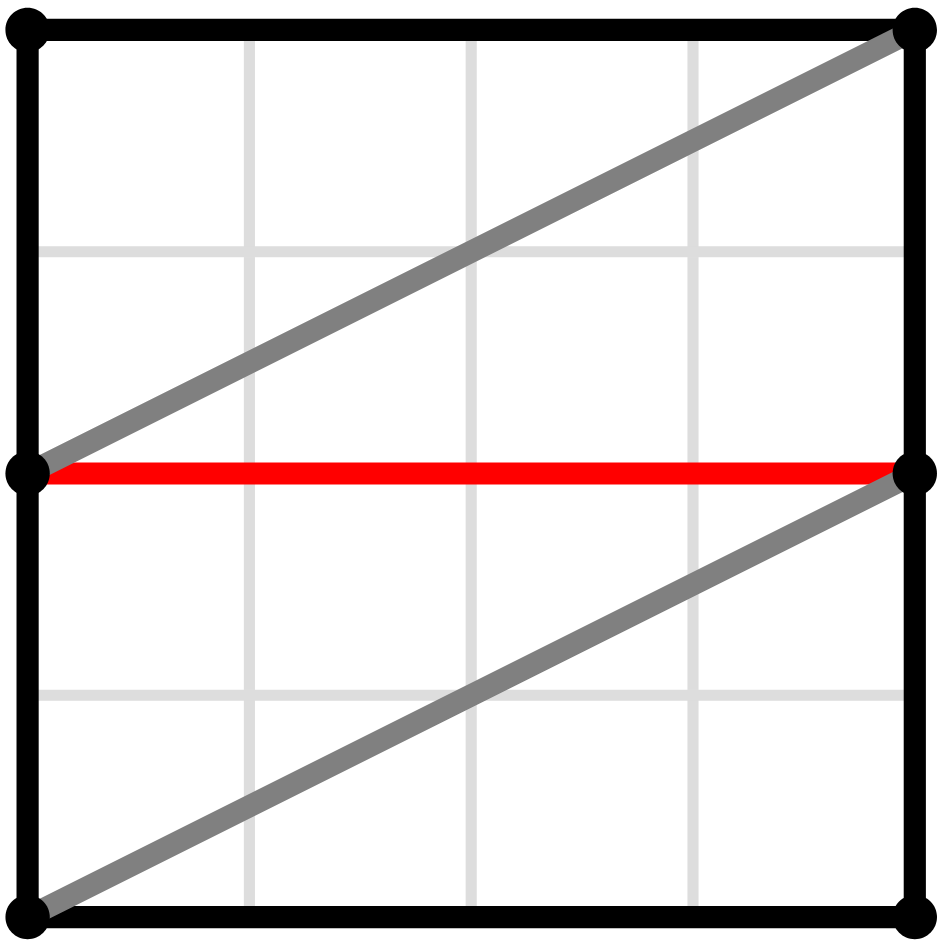
\includegraphics[width=.4\linewidth]{assets/3-2d-cp-triangulated.png} }}
\end{figure}

As an input, we get a set of 3D points, but triangulation works only in 2D.
Hence, at first we convert a set of 3D points to 2D by removing one of the axes (the one which will not lead to degenerate faces, if possible).
Then, 2D \textbf{Delaunay triangulation} is carried out (we used \textit{Shapely} library for that).
The algorithm introduces new edges. These edges are dynamically constrained to stay flat while folding.

There are cases, where the default triangulation will not be satisfactory
since we would like to preserve faces' concavity and the algorithm always generates a convex polygon.

\begin{figure}[H]
	\caption{An example, where triangulating a polygon marked with blue will result in an excessive triangle generated.}
	\centering
	\subfloat{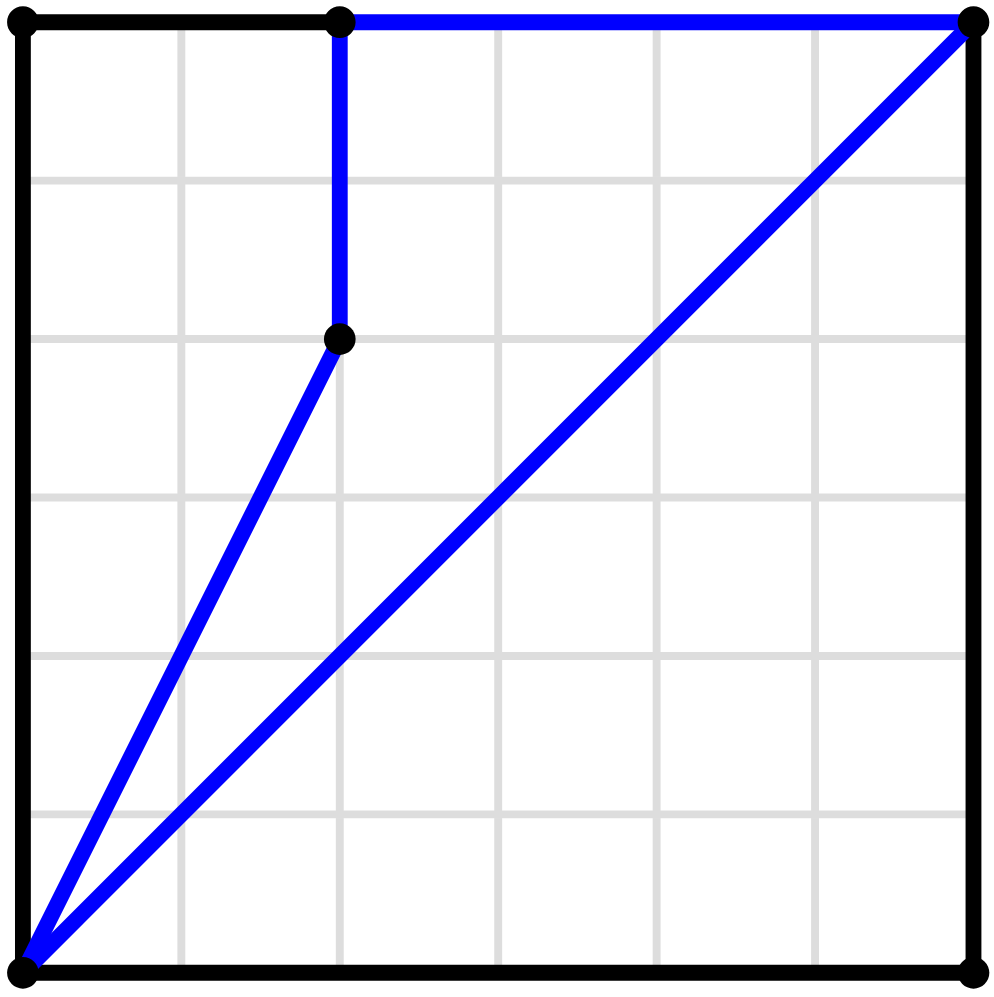
\includegraphics[width=0.5\textwidth]{assets/3-triangulation-improper-cp.png}}\qquad\qquad\qquad
	\subfloat[\centering Wrong (convex) triangulation]{{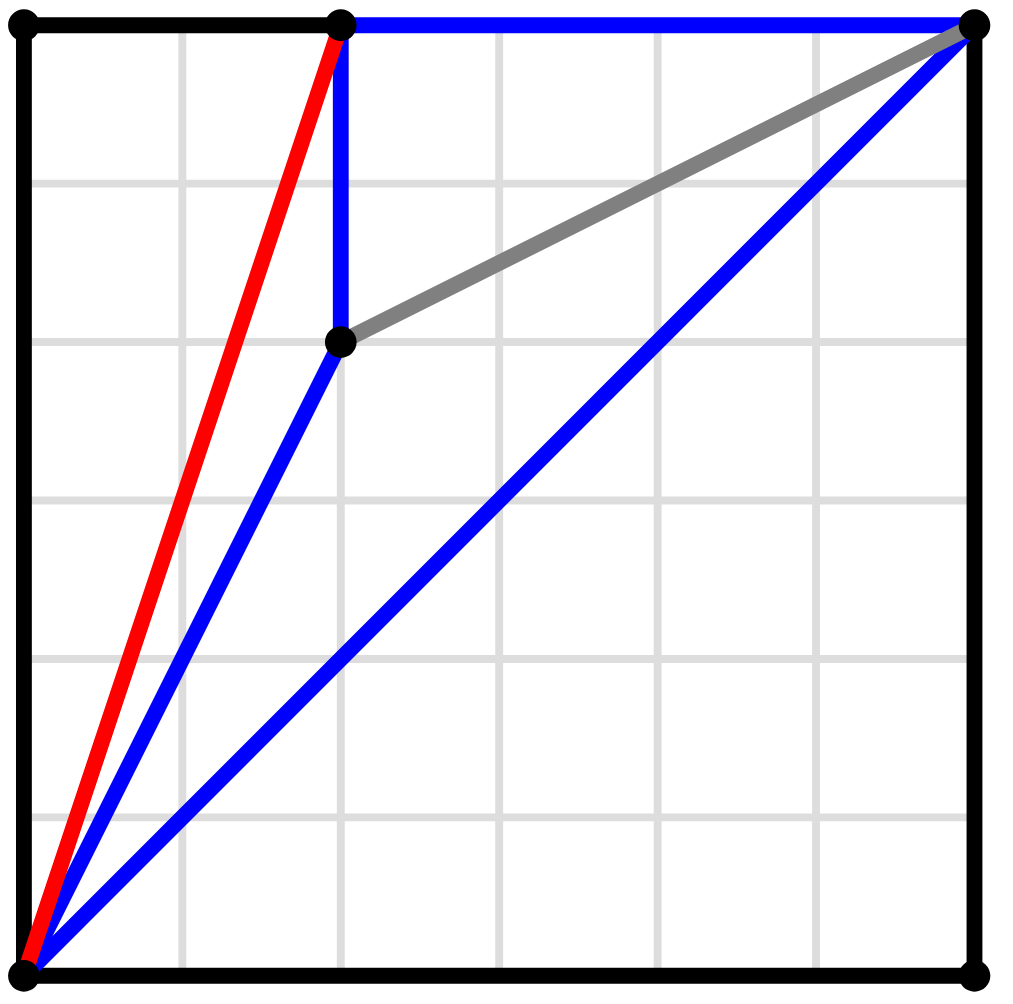
\includegraphics[width=.4\linewidth]{assets/3-triangulation-improper-cp-wrong.png} }}\qquad
	\subfloat[\centering Correct (concave) triangulation]{{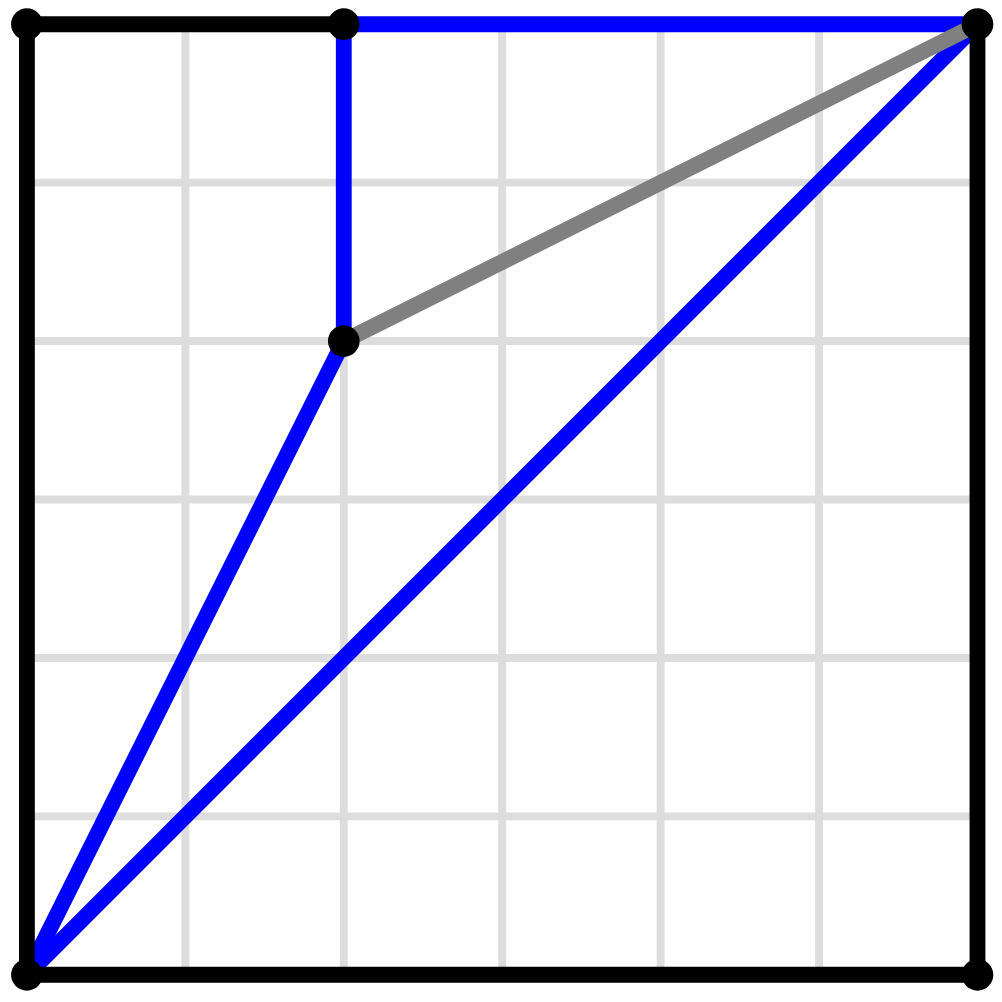
\includegraphics[width=.4\linewidth]{assets/3-triangulation-improper-cp-right.png} }}
\end{figure}

For such cases, we first compute a face's original hull. After the triangulation, we check whether the resulting triangles
lay within the original hull. If they do not, they are excluded from the triangulation result.

\smallskip
\textbf{Axial constraints - beam force}
\smallskip

Axial constraints prevent stretching and compression of edges. 
Each edge is modeled as a spring which length should be kept constant at each iteration.

\begin{figure}[H]
	\caption{Visualization of edge modeling}
    \centering
	\subfloat[\centering Edge modeled as a spring]{{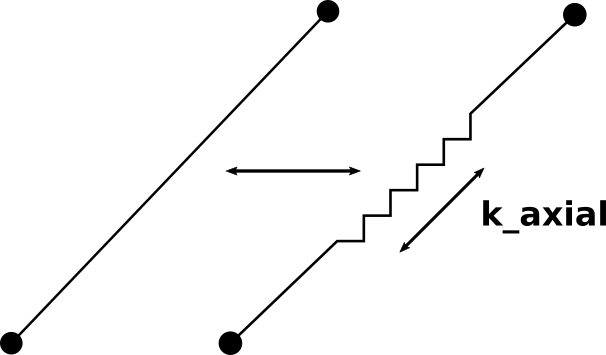
\includegraphics[width=.4\linewidth]{assets/3-edge_as_spring.png} }}
    \qquad
	\subfloat[\centering Axial constraints visualized ]{{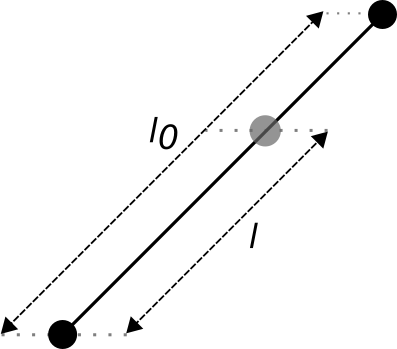
\includegraphics[width=.26\linewidth]{assets/3-edge_as_spring_l0_l.png} }}
\end{figure}

Before solving begins, the initial edge length $l_{0}$ is calculated.
Then, \textbf{Hooke's law} is used to calculate the beam force:

$$F_{l} = -k_{axial} * (l - l_{0})$$

where $l$ is the current edge length and $k_{axial}$ is a constant.

\smallskip
Before we apply the force to the vertices, first we need to convert it to a vector $\pmb{F}_{beam}$ in a model's coordinate space.
The $\pmb{F}_{beam}$ is related to the vertices position $\pmb{p}$ by:

$$\pmb{F}_{beam} = -\nabla V(\pmb{p}) = -\frac{\partial V}{\partial \pmb{p}}$$

where V is the potential energy of the system. By the chain rule, we get:

\begin{equation} \label{solver:beam_force}
\pmb{F}_{beam} = -\frac{\partial V}{\partial l}\frac{\partial l}{\partial \pmb{p}} = F_{l}\frac{\partial l}{\partial \pmb{p}} = -k_{axial} * (l - l_{0})\frac{\partial l}{\partial \pmb{p}}
\end{equation}


For the two vertices attached to the edge, we have:

$$ \frac{\partial l}{\partial \pmb{p_{1}}} = -\uveci_{12}, \frac{\partial l}{\partial \pmb{p_{2}}} = \uveci_{12} $$

where
\begin{itemize}
	\item $\uveci_{12}$ is a unit vector from vertex 1 to vertex 2
	\item $\pmb{p_{1}}$ is vertex 1 position
	\item $\pmb{p_{2}}$ is vertex 2 position
\end{itemize}

Although axial stiffness $k_{axial}$ could be related to material properties, we devised it experimentally.

All of this boils down to a few lines of code:

\lstinputlisting[language=Python]{assets/listings/beam_force.py}


\medskip
\textbf{Crease constraints - crease force}

With axial constraints we restrict the model to retain its shape while folding.
However, the main force that drives folding process is the result of crease constraints.
\smallskip

We drive faces connected by an edge to fold towards some target fold angle $\theta$.
The angle $\theta$ is the supplement of the dihedral angle between the two neighbouring triangular faces.

\begin{figure}[H]
	\caption{Crease constraints formulation between the two neighbouring triangular faces}
    \centering
	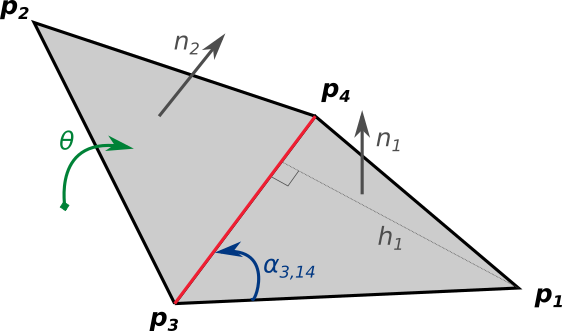
\includegraphics[width=.6\linewidth]{assets/3-crease_force_face.png}
	\label{solver:crease_force_face}
\end{figure}

Crease constraints are modeled as linear-elastic torsional springs.
Therefore, similarly to equation \eqref{solver:beam_force}, crease constraints will apply forces to the neighbouring
vertices by:

\begin{equation} \label{solver:crease_force}
	\pmb{F}_{crease} = -k_{crease}(\theta - \theta _{target})\frac{\partial \theta}{\partial \pmb{p}}
\end{equation}

where:

\begin{itemize}
	\item $\pmb{F}_{crease}$ is a force applied to a vertex in a model's coordinate space
	\item $k_{crease}$ is an edge folding stiffness (more on that below)
	\item $\theta$ is the current angle between the two faces (strictly speaking, supplement of the dihedral angle between the faces)
	\item $\theta _{target}$ is the desired angle between the two faces
\end{itemize}

In the implementation, there are 5 possible edge assignments:

\begin{enumerate}
	\item valley
	\item mountain
	\item flat
	\item boundary
	\item unknown
\end{enumerate}

$k_{crease}$ depends on the edge type.

The following piece of code computes the correct $k_{crease}$:

\lstinputlisting[language=Python]{assets/listings/crease_force_edge_assignment.py}

Let's introduce symbols:
\begin{itemize}
	\item $k_{fold} =$ \lstinline{CONFIG['FOLD_STIFFNESS']}
	\item $k_{facet} = $ \lstinline{CONFIG['FACET_STIFFNESS']}
\end{itemize}

As one can notice, the stiffness will be proportional to the initial edge length.
The stiffness parameter is chosen so that $k_{axial} \gg k_{fold}$.

Manipulating $k_{facet}$ influences how the material behaves. The smaller it is the more it acts like a piece of fabric.
The bigger it gets the more it starts to resemble paper and then plastic or metal.
\smallskip

As well as $k_{crease}$, angle $\theta _{target}$ also depends on the edge type:

$$
\theta _{target} =
\begin{cases}
	< 0 & \quad \text{for a mountain crease}\\
	> 0 & \quad \text{for a valley crease}\\
	0 & \quad \text{otherwise}
\end{cases}
$$

By default, the target angle will be one of: $\pi, -\pi, 0$ but the provided Instruction can override the default target angle.
\smallskip

Finally, partial derivatives of $\theta$ with respect to $\pmb{p}$ are given by:

\begin{equation} \label{solver:crease_force1}
\frac{\partial \theta}{\partial \pmb{p}_1} = \frac{\pmb{n}_1}{h_1}
\end{equation}

\begin{equation} \label{solver:crease_force2}
\frac{\partial \theta}{\partial \pmb{p}_2} = \frac{\pmb{n}_2}{h_2}
\end{equation}

\begin{equation} \label{solver:crease_force3}
	\frac{\partial \theta}{\partial \pmb{p}_3} = \frac{-\cot{\alpha _{4,31}}}{\cot{\alpha _{3,14}} + \cot{\alpha _{4,31}}} \frac{\pmb{n}_1}{h_1} + \frac{-\cot{\alpha _{4,23}}}{\cot{\alpha _{3,42}} + \cot{\alpha _{4,23}}} \frac{\pmb{n}_2}{h_2} 
\end{equation}

\begin{equation} \label{solver:crease_force4}
\frac{\partial \theta}{\partial \pmb{p}_4} = \frac{-\cot{\alpha _{3,14}}}{\cot{\alpha _{3,14}} + \cot{\alpha _{4,31}}} \frac{\pmb{n}_1}{h_1} + \frac{-\cot{\alpha _{3,42}}}{\cot{\alpha _{3,42}} + \cot{\alpha _{4,23}}} \frac{\pmb{n}_2}{h_2} 
\end{equation}

with all the symbols as marked on the figure \ref{solver:crease_force_face}.
\smallskip

The code for calculating crease force strictly follows the above formulations with one slight
addition - conditionally adding or subtracting a full angle if the faces passed through each other.
This prevents neighbouring faces from interpenetrating while folding.

\begin{figure}[H]
	\caption{Code that prevents faces from interpenetrating while folding}
	\lstinputlisting{assets/listings/crease_force_prevent_interpenetration.py}
\end{figure}

\medskip
\textbf{Face constraints - face force}
\smallskip

While not strictly necessary, face constraints add an additional layer of stability to the 
solving process. The face constraints are meant to keep interior angles of a face
constant during the folding process.

\begin{figure}[H]
	\caption{Face constraints add an additional force preventing faces from degeneration}
    \centering
	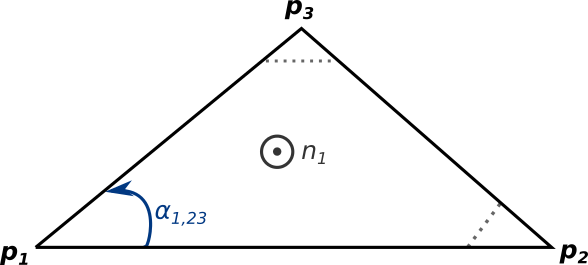
\includegraphics[width=.6\linewidth]{assets/3-face_force_face.png}
\end{figure}

As previously, face constraints are modeled as a linear-elastic spring.
For each of the interior angle of a triangular face, forces are applied to its neighbouring vertices.

\begin{equation} \label{solver:face_force}
	\pmb{F}_{face} = -k_{face}(\alpha - \alpha _0)\frac{\partial \alpha}{\partial \pmb{p}}
\end{equation}

where

\begin{itemize}
	\item $k_{face}$ is a face stiffness
	\item $\alpha$ is a current interior angle
	\item $\alpha _0$ is an initial interior angle
\end{itemize}

Derivatives of $\alpha$ with respect to $p$ are given by

\begin{equation} \label{solver:face_force1}
	\frac{\partial \alpha _{2,31}}{\partial \pmb{p}_1} = \frac{\pmb{n} \times (\pmb{p}_1 - \pmb{p}_2)}{\norm{\pmb{p}_1 - \pmb{p}_2}^2}
\end{equation}

\begin{equation} \label{solver:face_force2}
	\frac{\partial \alpha _{2,31}}{\partial \pmb{p}_2} = \frac{\pmb{n} \times (\pmb{p}_1 - \pmb{p}_2)}{\norm{\pmb{p}_1 - \pmb{p}_2}^2} + \frac{\pmb{n} \times (\pmb{p}_3 - \pmb{p}_2)}{\norm{\pmb{p}_3 - \pmb{p}_2}^2}
\end{equation}

\begin{equation} \label{solver:face_force3}
	\frac{\partial \alpha _{2,31}}{\partial \pmb{p}_3} = \frac{\pmb{n} \times (\pmb{p}_3 - \pmb{p}_2)}{\norm{\pmb{p}_3 - \pmb{p}_2}^2}
\end{equation}


\medskip
\textbf{Damping - damping force}
\smallskip

Damping is an additional force that is not required from the modeling perspective
but is required from the solver's stability point of view. It prevents model's
oscillation while folding and without it barely any model folds correctly.

\begin{figure}[H]
	\caption{Damping force formulation on the two vertices connected by an edge}
    \centering
	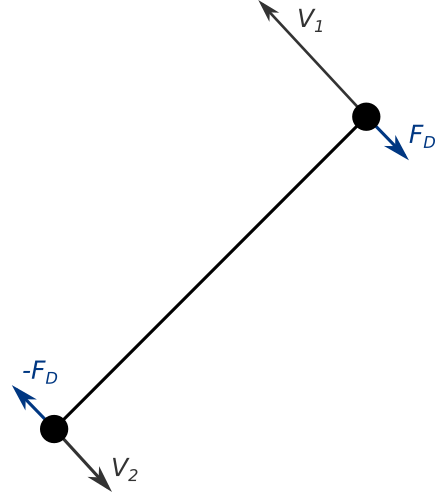
\includegraphics[width=.4\linewidth]{assets/3-damping_force_edge.png}
\end{figure}

Damping force is defined in terms of vertices' velocity as:


$$F_{damping} = -e_{damping} * (V_1 - V_2)$$

where:

\begin{itemize}
	\item $e_{damping}$ is a damping coefficient 
	\item $V_1$ and $V_2$ are vertices' velocities
\end{itemize}

For each edge damping coefficient is set as:

$$ e_{damping} = d_p * 2 * \sqrt{k_{axial} * min(v1_{mass}, v2_{mass})} $$

where:

\begin{itemize}
	\item $d_p$ is a configurable damping percent
	\item $k_{axial}$ is axial stiffness defined previously
	\item $vx_{mass}$ is mass of a vertex $x$
\end{itemize}

We assume that mass is constant for each vertex.

As is the case for beam force, damping force is computed in a model's coordinate space
and then applied to each of the edge's vertices.
\smallskip

\begin{figure}[H]
	\centering
	\caption{The code carrying out damping force calculation}
	\lstinputlisting{assets/listings/damping_force.py}
\end{figure}

\medskip
\textbf{Numerical integration}
\smallskip

Once all the forces are defined, the total force for each vertex is computed as a sum of all the imposed forces.

\begin{equation} \label{solver:total_force}
	\pmb{F}_{total} = \sum_{edges} \pmb{F}_{beam} + \sum_{edges} \pmb{F}_{crease} + \sum_{faces}\pmb{F}_{face} + \sum_{edges}\pmb{F}_{damping}
\end{equation}

Then using Newton's Second Law of Dynamics we compute acceleration as:

$$
\pmb{a} = \frac{\pmb{F}_{total}}{m}
$$

where $m$ is a vertex's mass. We assumed that mass is constant for each vertex, however a more appropriate analysis could yield
better results in terms of folding dynamics.

Having acceleration, we compute vertex velocity, and next position using \textit{forward Euler Integration} method:

$$
\begin{aligned}
\pmb{V}_{t+\Delta t} = \pmb{V}_t + \pmb{a}\Delta t \\
\pmb{p}_{t+\Delta t} = \pmb{p}_t + \pmb{V}\Delta t
\end{aligned}
$$

We assume the initial conditions:

\begin{equation}
	\begin{aligned}
		\pmb{V}_0 = 0\\
		\pmb{p}_0 = \text{provided by Instruction}
	\end{aligned}
\end{equation}


As an end condition, we check whether the difference between current and previous forces is smaller than some configured $\varepsilon$:

\begin{lstlisting}[language=Python]
diff = np.abs(np.array(current_forces) - np.array(previous_forces))
return np.all(diff <= epsilon)
\end{lstlisting}

To generate all the Transitions in the model, we run the solve function for each step in the Instruction.

\begin{figure}[H]
	\caption{The simplified pseudocode for the solving process}
	\lstinputlisting{assets/listings/solver.py}
\end{figure}


\subsection{Development environment setup}
% Instrukcja postawienia środowiska deweloperskiego - jeśli potrzeba wypełniacza %

\subsection{Deployment}
% Instrukcja postawienia środowiska deweloperskiego - jeśli potrzeba wypełniacza %

\subsection{Quality assurance}
% Quality Assurance: czy mamy testy jednostkowe? Czy mamy inne testy automatyczne? Jakich bibliotek używacie? %
At every commit that is a part of the master branch or a Pull Request Unit Tests are run. \\

\subsection{Problems encountered}
% Z jakimi problemami technicznymi sie borykaliście? Jeśli nie opisaliście ich w dokumentacji procesowej. %

